\documentclass[12pt,tiks]{article}
\usepackage[utf8]{inputenc}
\usepackage[OT1]{fontenc}
\usepackage[american]{babel}
\usepackage{ragged2e}
\usepackage{layout} 
\usepackage{csquotes}
\usepackage[expansion,babel=true]{microtype}
\usepackage{layout}
\usepackage{xpatch}
\usepackage{titling}
\usepackage[affil-it]{authblk}
\usepackage{hyperref}
\usepackage{comment}
\usepackage{caption}
\usepackage{pbox}
\usepackage{fancyhdr}
\usepackage{setspace}
\usepackage{tabularx}
\usepackage{sectsty}
\usepackage[most]{tcolorbox}
\usepackage{enumerate}
\usepackage[dvipsnames]{xcolor}
\usepackage[noeepic]{qtree}
\usepackage{tikz}
\usepackage{tkz-euclide}
\usetikzlibrary{arrows.meta,calc,intersections}
\usepackage{mathtools}
\usepackage{bm}
\usepackage{esvect}
\usepackage{blkarray, bigstrut}
\usepackage{gauss}
\usepackage{systeme}

\newcommand{\icol}[1]{% inline column vector
  \left(\begin{smallmatrix}#1\end{smallmatrix}\right)%
}

\makeatletter
\renewcommand*\env@matrix[1][*\c@MaxMatrixCols c]{%
  \hskip -\arraycolsep
  \let\@ifnextchar\new@ifnextchar
  \array{#1}}
\makeatother

\pagestyle{fancy}
\fancyhf{}
\rhead{Page \thepage}
\chead{Introduction to Matrices}
\lhead{Algebra 2}
\lfoot{George Ranch High School}
\rfoot{\today}
\cfoot{Lamar CISD}


\begin{document}
\pagestyle{plain}
\pagenumbering{gobble}
\section*{Introduction to Matrices: Notes \& Practice}
    \subsubsection*{\textit{What Is a Matrix?}}
        \begingroup{
        \begin{minipage}[t][.5in][t]{2.5in}\RaggedRight
        Instead of starting with a lengthy or scary definition, let's just look at a simple single column matrix:
        \end{minipage}
        \hspace{.1in}
        \begin{minipage}[t][.5in][t]{1in}\vspace{-1.75em}
        $\vv{X}=
        \stackrel{\mbox{$x_{i,j}$}}{%
        \vspace{.3em}
        \begin{bmatrix}
        3\\
        4\\
        5\\
        \end{bmatrix}%
        }
        $
        \end{minipage}
        \begin{minipage}[t][.5in][t]{1.75in}\vspace{-.20in}\RaggedRight{
        \footnotesize{This is a single column matrix consisting only of $x$ values. Matrix letter names are \textbf{\textit{always capitalized}}.}}
        \end{minipage}
        }
    
    \vspace{-.15in}
    
    \subsubsection*{Describing Matrices\footnote{$\;$ Matrices: \textit{(n.)} plural form of matrix; pronounced ``may-treh-sees".}}
        \begin{minipage}[t][2in][t]{2.75in}
        \Centering{\textbf{Rows \& Columns}}
        \newline 
        \justifying{
        \onehalfspacing\footnotesize{One refers to matrices first by row, then by column; therefore, $\vv{X}$ is a three row by one column matrix or a \textit{3 by 1} matrix. \textit{Row} positions are denoted by the subscript $i$ and \texit{columns} are denoted by the subscript $j$. For example, the $4$ in the $\vv{X}$ matrix above has an $i$ position of $2$ and a $j$ position of $1$; therefore, its position in $\vv{X}$ is $\coords{i,j}$ or $\coords{2,1}$.}}
        \end{minipage} 
        \hspace{.1in}\rule[-1.65in]{.01in}{1.75in}\hspace{.1in}
        \begin{minipage}[t][2in][t]{2.5in}
        \Centering{\textbf{Vector Notation}}
        \newline 
        \justifying{
        \onehalfspacing\footnotesize{The $\bm{\rightarrow}$ arrow above the capital $X$ means $\vv{X}$ is called a single column \textit{vector} matrix because  $\vv{X}=\icol{3\\4\\5}$ refers to a \textit{vector}: a quantity with both \textit{magnitude} and \textit{direction}. $\vv{X}$ may also be written in row form as $\vv{X}=\icol{3_x,4_y,5_z}$. Both column and row forms of $\vv{X}$ are plotted below to show how they relate.}}
        \end{minipage}
        
        \vspace{-.325in}
        
    \subsubsection*{Graphing Matrices}
        \RaggedRight \small{Now we will geometrically plot the $\vv{X}$ matrix in column form as three values of $x$ and row form as values of $x$, $y$, and $z$, then compute the vector's \textit{magnitude}\footnote{$\;$ The \textit{magnitude} (also called the \textit{norm}) of $\vv{X}$ is written $|{\vv{X}}|=\sqrt{3^{2}+4^{2}+5^{2}}=\sqrt{50}=5\sqrt{2}$ which is also \textbf{the length of each of the hypotenuses} of the right triangles pictured above.}.}
        \vspace{.05in}
        
        \begin{minipage}[t][2in][t]{2.7in}
        \Centering{\small{Column Vector Matrix $\vv{X}=\icol{3_{x_1}\\4{x_2}\\5{x_3}}$}}
        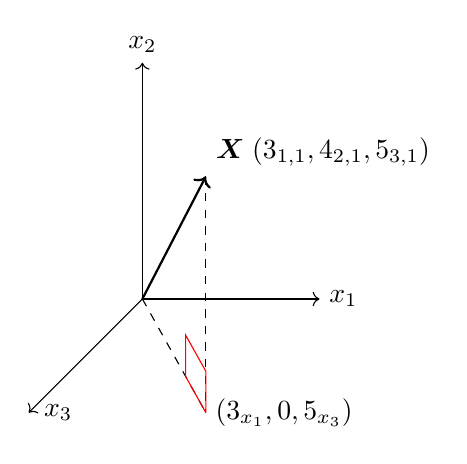
\begin{tikzpicture}[scale=.75]
            \coordinate (O) at (0,0,0);
            \coordinate (A) at (3,0,0);
            \coordinate (B) at (0,4,0);
            \coordinate (C) at (0,0,5);
            \coordinate (D) at (3,4,5);
            \coordinate (E) at (3,0,5);
            \coordinate (x) at (3,0,0);
            \coordinate (y) at (0,4,0);
            \coordinate (z) at (0,0,5);
            \draw[->] (O)--(x) node[right]{$x_1$};
            \draw[->] (O)--(y) node[above]{$x_2$};
            \draw[->] (O)--(z) node[right=2pt]{$x_3$};
            \draw[->,thick] (O)--(D) node[above right]{$\vv{\bm{X}}\;\coord(3_{1,1},4_{2,1},5_{3,1})$};
            \draw[dashed] (O)--(E) node[right]{$\coord(3_{x_1},0,5_{x_3})$};
            \draw[dashed] (D)--(E);
            \tkzMarkRightAngle[draw=red,size=.7](D,E,O);
            % \tkzLabelAngle[dist=-.25](D,E,O){$E$};
        \end{tikzpicture}
        \end{minipage}
        \hspace{.2in}
        \begin{minipage}[t][2in][t]{2.7in}
        \Centering{\small{Row Vector Matrix $\vv{X}=\icol{3_{x},4_{y},5_{z}}$}}
        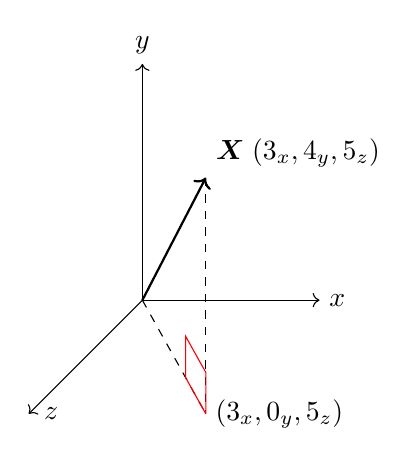
\begin{tikzpicture}[scale=.75]
            \coordinate (O) at (0,0,0);
            \coordinate (A) at (3,0,0);
            \coordinate (B) at (0,4,0);
            \coordinate (C) at (0,0,5);
            \coordinate (D) at (3,4,5);
            \coordinate (E) at (3,0,5);
            \coordinate (x) at (3,0,0);
            \coordinate (y) at (0,4,0);
            \coordinate (z) at (0,0,5);
            \draw[->] (O)--(x) node[right]{$x$};
            \draw[->] (O)--(y) node[above]{$y$};
            \draw[->] (O)--(z) node[right=2pt]{$z$};
            \draw[->,thick] (O)--(D) node[above right]{$\vv{\bm{X}}\;\coord{(3_{x},4_{y},5_{z}})$};
            \draw[dashed] (O)--(E) node[right]{$\coord(3_x,0_y,5_z)$};
            \draw[dashed] (D)--(E);
            \tkzMarkRightAngle[draw=red,size=.7](D,E,O);
            % \tkzLabelAngle[dist=-.25](D,E,O){$E$};
        \end{tikzpicture}
        \end{minipage}
        
\vspace*{\fill}
\newpage
\clearpage
\thispagestyle{fancy}
\pagenumbering{arabic}
\setcounter{page}{2}
    \subsection*{Converting Systems of Equations to Matrices}
       \begin{minipage}[t][.5in][t]{2.4in}\RaggedRight
        Consider the following system of two simultaneous linear equations. How might you convert these equations into matrix form?
            \begin{equation*}
              \systeme{
                      -8x-3y=-19,
                      16x-8y=24
                      }
            \end{equation*}
        \end{minipage}
        \hspace{.2in}
        \begin{minipage}[t][.5in][t]{2.4in}\RaggedRight
        In order to convert those equations into a matrix we must strip away the letters and use a matrix form called an \textit{augmented matrix}:
        \-\vspace*{.15in}
        $
            \begin{bmatrix}[*1cr@{\quad}|@{\quad}>{\color{black}}r]
              -8 & -3 & -19 \\
              16 & -8 & 24
            \end{bmatrix}
        $
        \end{minipage}
        
    \-\hspace*{\fill}
    \-\vspace*{1in}
    \subsection*{How to Solve Systems Using Gaussian Elimination}
    Focus on the \textbf{left side} of that augmented matrix for a minute.
    \par\vspace{.05in}
    \begin{minipage}[t][.5in][t]{2.4in}\RaggedRight
    What you want to do is play around with the \textit{rows} of that augmented matrix until the four numbers on the left side look like this:
    \end{minipage}
    \hspace{.1in}
    \begin{minipage}[t][.5in][t]{1in}\RaggedRight
    \par\vspace{.05in}\hspace{.15in}
        $
        \begin{bmatrix}
          1 & 0 \\
          0 & 1
        \end{bmatrix}
        $
    \end{minipage}
    \hspace{.1in}
    \begin{minipage}[t][.5in][t]{2.4in}\RaggedRight
    This is called an \textbf{identity matrix}. If you can make the \textit{left side} of your matrix look like this, you will have \textbf{solved it} for \textit{both variables}.
    \end{minipage}
    
    \-\hspace*{\fill}
    \-\vspace*{.15in}
    
    \textbf{How do you do this?} You manipulate the \textit{entire rows} using what are called \textit{elementary row operations}. \textbf{This is \textit{much easier} than it looks}. Watch this:
    
    \par\vspace{.05in}
    
    \begin{minipage}[t][.5in][t]{2.5in}\RaggedRight
    Here is our augmented matrix again:
    
    \par\vspace{.05in}
    
        $
            \begin{bmatrix}[*1cr@{\quad}|@{\quad}>{\color{black}}r]
              -8 & -3 & -19 \\
              16 & -8 & 24
            \end{bmatrix}
        $
    \end{minipage}
    \hspace{.1in}
    \begin{minipage}[t][.5in][t]{2.4in}\RaggedRight
    What if we divided \textit{the entire bottom row} by $2$ then added it to the top row, replacing the bottom row with the resulting sum?
    \end{minipage}
    
    \hspace{.1in}\vspace{.5in}
    
    \begin{minipage}[t][.5in][t]{2.4in}\RaggedRight
    \textbf{Step 1}: Divide the whole bottom row by $2$:
    
    \par\vspace{.05in}
    
        $
            \begin{bmatrix}[*1cr@{\quad}|@{\quad}>{\color{black}}r]
              -8 & -3 & -19 \\
              \frac{16}{2} & \frac{-8}{2} & \frac{24}{2}
            \end{bmatrix}
        $
    \end{minipage}
    \hspace{.1in}
    \begin{minipage}[t][.7in][t]{3in}\RaggedRight
    \-\vspace*{.1in}
    \textbf{Step 2}: (intermediate step): Simplify.
    
    \par\vspace{.05in}
    
        $
            \begin{bmatrix}[*1cr@{\quad}|@{\quad}>{\color{black}}r]
              -8 & -3 & -19 \\
              8 & -4 & 12
            \end{bmatrix}
        $
    \end{minipage}
    
    \hspace{.1in}\vspace{.5in}
    
    \begin{minipage}[t][.7in][t]{3in}\RaggedRight
    \-\vspace*{.1in}
    \textbf{Step 3}: Add \textit{new} bottom row to top row:
        $
            \begin{bmatrix}[*1cr@{\quad}|@{\quad}>{\color{black}}r]
              -8 & -3 & -19 \\
              ({8+{-8}}) & ({-4+{-3}}) & ({12+{-19}})
            \end{bmatrix}
        $
    \end{minipage}
    \hspace{.1in}
    \begin{minipage}[t][.7in][t]{3in}\RaggedRight
    \-\vspace*{.1in}
    \textbf{Step 4}: (intermediate step): Simplify.
        $
            \begin{bmatrix}[*1cr@{\quad}|@{\quad}>{\color{black}}r]
              -8 & -3 & -19 \\
              0 & -7 & 7
            \end{bmatrix}
        $
    \end{minipage}
    
    \hspace{.1in}\vspace{.5in}
\newpage
\clearpage
\thispagestyle{fancy}
    \begin{minipage}[t][.7in][t]{3in}\RaggedRight
    \-\vspace*{.1in}
    \textbf{Step 5}: Divide \textit{entire bottom row} by $-7$.
        $
            \begin{bmatrix}[*1cr@{\quad}|@{\quad}>{\color{black}}r]
              -8 & -3 & -19 \\
              \frac{0}{-7} & \frac{-7}{-7} & \frac{7}{-7}
            \end{bmatrix}
        $
    \end{minipage}
    \hspace{.1in}
    \begin{minipage}[t][.7in][t]{3in}\RaggedRight
    \-\vspace*{.1in}
    \textbf{Step 6}: (intermediate step): Simplify.
     $
            \begin{bmatrix}[*1cr@{\quad}|@{\quad}>{\color{black}}r]
              -8 & -3 & -19 \\
              0 & 1 & 1
            \end{bmatrix}
        $
    \end{minipage}
    
    \hspace{.1in}\vspace{.5in}
    
    \begin{minipage}[t][.7in][t]{3in}\RaggedRight
    \-\vspace*{.1in}
    \textbf{Step 7}: Add the bottom row to the top.
        $
            \begin{bmatrix}[*1cr@{\quad}|@{\quad}>{\color{black}}r]
              ({-8+0}) & ({-3+1}) & ({-19+1}) \\
              0 & 1 & 1
            \end{bmatrix}
        $
    \end{minipage}
    \hspace{.1in}
    \begin{minipage}[t][.7in][t]{3in}\RaggedRight
    \-\vspace*{.1in}
    \textbf{Step 8}: (intermediate step): Simplify.
        $
            \begin{bmatrix}[*1cr@{\quad}|@{\quad}>{\color{black}}r]
              -8 & -2 & -18 \\
              0 & 1 & 1
            \end{bmatrix}
        $
    \end{minipage}
    
    \hspace{.1in}\vspace{.5in}
    
    \begin{minipage}[t][.7in][t]{3in}\RaggedRight
    \-\vspace*{.1in}
    \textbf{Step 9}: Divide top row by $-2$.
     $
            \begin{bmatrix}[*1cr@{\quad}|@{\quad}>{\color{black}}r]
              \frac{-8}{-2} & \frac{-2}{-2} & \frac{-18}{-2} \\
              0 & 1 & 1
            \end{bmatrix}
        $
    \end{minipage}
    \hspace{.1in}
    \begin{minipage}[t][.7in][t]{3in}\RaggedRight
    \-\vspace*{.1in}
    \textbf{Step 10}: (intermediate step): Simplify.
        $
            \begin{bmatrix}[*1cr@{\quad}|@{\quad}>{\color{black}}r]
              4 & 1 & 9 \\
              0 & 1 & 1
            \end{bmatrix}
        $
    \end{minipage}
    
    \hspace{.1in}\vspace{.5in}
    
    \begin{minipage}[t][.7in][t]{3in}\RaggedRight
    \-\vspace*{.1in}
    \textbf{Step 11}: Subtract the bottom row from the top.
        $
            \begin{bmatrix}[*1cr@{\quad}|@{\quad}>{\color{black}}r]
              ({4-0}) & ({1-1}) & ({9-1}) \\
              0 & 1 & 1
            \end{bmatrix}
        $
    \end{minipage}
    \hspace{.1in}
    \begin{minipage}[t][.7in][t]{3in}\RaggedRight
    \-\vspace*{.1in}
    \textbf{Step 12}: (intermediate step): Simplify.
        $
            \begin{bmatrix}[*1cr@{\quad}|@{\quad}>{\color{black}}r]
              4 & 0 & 8 \\
              0 & 1 & 1
            \end{bmatrix}
        $
    \end{minipage}
    
    \hspace{.1in}\vspace{.5in}
    
    \begin{minipage}[t][.7in][t]{3in}\RaggedRight
    \-\vspace*{.1in}
    \textbf{Step 13}: Divide the top row by $4$.
        $
            \begin{bmatrix}[*1cr@{\quad}|@{\quad}>{\color{black}}r]
              \frac{4}{4} & \frac{0}{4} & \frac{8}{4} \\
              0 & 1 & 1
            \end{bmatrix}
        $
    \end{minipage}
    \hspace{.1in}
    \begin{minipage}[t][.7in][t]{3in}\RaggedRight
    \-\vspace*{.1in}
    \textbf{FINAL STEP}: Simplify. You're done!
        $
            \begin{bmatrix}[*1cr@{\quad}|@{\quad}>{\color{black}}r]
              1 & 0 & 2 \\
              0 & 1 & 1
            \end{bmatrix}
        $
    \end{minipage}
    
    \hspace{.1in}\vspace{.3in}
    
    Since the left side is the \textbf{identity matrix} ${I}=\icol{1 & 0 \\ 0 & 1}$ then $x=2$ and $y=1$. Thus, the solution to the system of equations is $(\coord{2,1})$.
    
    \par\vspace{.1in}
    You just performed something \textsc{amazing} called \textit{Gaussian elimination} in order to reduce the original augmented matrix to a new form called \textbf{reduced row echelon form}. This technique was invented by Carl Friedrich Gauss (1777–1855). It's \textit{extraordinarily powerful} in what it can do with \texttt{really simple arithmetic}. 
    
    \newpage
    \clearpage
    \thispagestyle{fancy}
    
    You can do the same operations on multiple additional equations, including two, three, or more multiple variable equations too!
    
    \hspace{.1in}\vspace{.05in}
    
    Here are the \textbf{three rules} of \textit{Gaussian elimination}:
    \begin{enumerate}
        \item You can multiply a row by a non-zero number (negative numbers and fractions are allowed).
        \item You can add one row to another row or to a multiple of another row.
        \item You can swap the positions of any two rows.
    \end{enumerate}
    
\section*{Now It's Your Turn!}
    \subsection*{Practice Questions to Gauge Understanding}
    \begin{minipage}[t][.7in][t]{3in}\RaggedRight
    \-\vspace*{.1in}
    \textbf{Question 1}: Convert the following system of two linear equations with two variables into an augmented matrix and write your answer in the blank space to the right:
        \begin{equation*}
          \systeme{
                  12x-3y=3,
                  3x-7y=24
                  }
        \end{equation*}
    \end{minipage}
    
    \hspace{.1in}\vspace{1in}
    
    \begin{minipage}[t][.7in][t]{3in}\RaggedRight
    \-\vspace*{.1in}
    \textbf{Question 2}: Convert the following system of three linear equations with three variables into an augmented matrix and write your answer in the blank space to the right:
        \begin{equation*}
          \systeme{
                  -2x + y + z = -5,
                  x + y + z = 4,
                  6x + 4y -3z = 8
                  }
        \end{equation*}
    \end{minipage}
    
    \hspace{.1in}\vspace{.5in}
    
    \newpage
    \clearpage
    \thispagestyle{fancy}
    
    \begin{minipage}[t][.7in][t]{3in}\RaggedRight
    \-\vspace*{.1in}
    \textbf{Question 3}: Identify the matrix element located at position $(\coord{i_2,j_3})$.
    
    \-\vspace*{.1in}
    
         $
            \begin{bmatrix}[*2cr@{\quad}|@{\quad}>{\color{black}}r]
              3 & -4 & 1 & -25 \\
              2 & 4 & 0 & -2 \\
              6 & 4 & -3 & 8
            \end{bmatrix}
        $
    \end{minipage}
    
    \hspace{.1in}\vspace{1in}
    
    \begin{minipage}[t][.7in][t]{3in}\RaggedRight
    \-\vspace*{.1in}
    \textbf{Question 4}: Which of the following are \textbf{true} about\textit{vectors}? (Circle all that apply.)
        \begin{enumerate}
            \item A. They can rotate freely about the $z$-axis.
            \item B. Vectors have a definite \textit{magnitude}.
            \item C. Vectors do not have any specific direction.
            \item D. Vectors were discovered by  Carl Friedrich Gauss (1777–1855)
            \item E. Vectors have a specific direction.
            \item F. The magnitude of a vector in three dimensions is equivalent to the hypotenuse of a right triangle formed by the origin, the distance from the origin to the intersection of the $x$ and $z$ values, and the intersection of the $x$, $y$, and $z$ values.
            \item G. Given the $(\coords{x,y,z})$ of the intersection of three planes is located at $(\coords{3,4,5})$, the magnitude of the vector is $5$.
            \item H. \textbf{This} is a vector: $\vv{B}=\icol{-5\\2\\9}$
        \end{enumerate}
    \end{minipage}
    \hspace{.1in}
     \begin{minipage}[t][.7in][t]{3in}\RaggedRight
        \-\vspace*{.1in}
        \textbf{Question 5}: Write down the three rules of Gaussian elimination in the blank space \textbf{above}. \textsc{optional additional \textbf{\textsc{bonus challenge}}}: Use Gaussian elimination to solve for $x$ and $y$ given the following system of two linear equations with two variables:
        \begin{equation*}
              \systeme{
                      -3x+10y=-8,
                      5x-20y=10
                      }
            \end{equation*}
    \end{minipage}
    
    \-\vspace*{\fill}
    
    \Centering\textsc{THANK YOU FOR COMPLETING THIS ASSIGNMENT.}
    
    
\end{document}

